
\begin{center}
\Huge
Mængder
\end{center}

\section*{Mængder}
\stepcounter{section}
Mængder er det af de mest fundamentale matematiske objekter, og de udgør de grundlæggende byggesten (aksiomer) i dem mest gængse opbygning af matematikken. Vi starter med en definition, der er præcis nok til vores forståelse.
\begin{defn}
En mængde er et matematisk objekt, der består af en samling af elementer. Hvis et element $a$ er indeholdt i en mængde $A$, skriver vi $a\in A$.
\end{defn} 
Hvis $A$ er en mængde med elementerne $a$, $b$ og $c$, så skriver vi $A$ som $A= \{a,b,c\}$, altså med krøllede parenteser (tuburg-parenteser), og elementerne separeret med kommaer. Eksempler på mængder er $\{2,4,6,8\}$ og $\{7,b,4\}$. En uendelig mængde noteres med ellipse $\hdots$. Det kunne eksempelvis være de lige tal $\{\hdots,-4,-2,0,2,4,\hdots\}$. Vi vil nu gennemgå en række vigtige eksempler:
\begin{exa}
Vi vil arbejde med følgende vigtige mængder:
\begin{enumerate}[label=\roman*)]
\item Der er en mængde, der ingen elementer har. Denne mængde kaldes den tomme mængde og noteres med $\emptyset$ eller $\{\}$. 
\item Mængden af naturlige tal $\mathbb{N} = \{0,1,2,3,\hdots\}$.
\item Mængden af hele tal $\mathbb{Z} = \{\hdots,-3,-2,-1,0,1,2,3,\hdots \}$.
\item Mængden af alle rationale tal/heltalsbrøker $\mathbb{Q} = \left\{\frac{a}{b} \ \middle | \ a,b\in \mathbb{Z}\right\}$. Eksempler er $1/2, 4, 27/3$
\item Mængden af reelle tal $\mathbb{R}$, der består af alle rationale tal og alle uendelige decimalfølger. Eksempler er $e,\pi, \sqrt{2}$
\end{enumerate}
\end{exa}
Hvis en mængde $A$ er indeholdt i en mængde $B$, så skriver vi $A\subseteq B$ og $A$ kaldes en delmængde af $B$. To mængder er ens, hvis de indeholder hinanden, altså $A\subseteq B$ og $B\subseteq A$ og vi skriver $A=B$. 
\begin{exa}
Vi har følgende eksempler på delmængder:
\begin{enumerate}[label=\roman*)]
\item Mængden af alle mennesker er en delmængde af alle pattedyr som igen er en delmængde af alle dyr.
\item $\{1,2,3\} \subseteq \{1,2,3,4\}$.
\item De lige tal er en delmængde af de hele tal.  
\item $\{10,20\}\subseteq \{10,20\}$.
\end{enumerate}
\end{exa}

\section*{Mængdeoperationer}
Har vi to mængder, kan vi gøre os overvejelser om, hvordan disse mængder kan sammenlignes, og hvordan vi kan danne nye mængde ud fra gamle. 
\begin{defn}[Fællesmængde]
Fællesmængden mellem to mængder $A$ og $B$ er den mængde, der består af de elementer, som begge mængder har til fælles. Mængden betegnes med
\begin{align*}
A\cap B
\end{align*}
og defineres mere præcist
\begin{align*}
A\cap B = \{a\in A, b\in B \mid a\in B, b\in A\}.
\end{align*}
\end{defn}

\begin{exa}
Eksempler på fællesmængder er:
\begin{enumerate}[label=\roman*)]
\item $\{1,2,3\} \cap {2,3,4} = \{2,3\}$.
\item $\{1,2,3\} \cap \{4,5,6\} = \emptyset$.
\item      $\{$Pattedyr$\}$ $\cap$ $\{$Havdyr$\}$ = $\{$Hvaler, Sæler, Søkøer, Isbjørne, Havoddere$\}$
\end{enumerate}
\end{exa}

\begin{defn}[Foreningsmængde]
Foreningsmængden af to mængder $A$ og $B$ består af de elementer, der er i enten $A$ eller $B$ og betegnes
\begin{align*}
A\cup B = \{a\in A, b\in B\}.
\end{align*}
\end{defn}
\begin{exa}
Vi har følgende eksempler på foreningsmængder:
\begin{enumerate}[label=\roman*)]
\item $\{1,2,3\} \cup \{4,5,6\} = \{1,2,3,4,5,6\}$.
\item $\{1,2\} \cup \{1,2,3,4\} = \{1,2,3,4\}$.
\item $\{$Ulige tal $\}$ $\cup$ $\{$Lige tal$\}=\mathbb{Z}$ 
\end{enumerate}
\end{exa}
\begin{defn}
Mængdedifferencen af to mængder $A$ og $B$ betegnes
\begin{align*}
A \backslash B
\end{align*}
og betegner de elementer, der er i $A$, men ikke i $B$. Bemærk at $A\backslash B$ og $B \backslash A$ generelt er forskellige.
\end{defn}

Vi har ofte brug for en mængde, der indeholder alle interessante elementer i en eller anden sammenhæng. Denne kaldes for universalmængden og betegnes med $U$. 
\begin{defn}
Komplementærmængden til en mængde $A$ betegnes med 
\begin{align*}
A^C 
\end{align*}
og defineres som $U\backslash A$. 
\end{defn}
\begin{exa}
Hvis $U$ består af mængden af udfald af et terningeslag $U=\{1,2,3,4,5,6\}$ og $A$ er mængden af udfald $A=\{1,2\}$, så vil komplementærmængden $A^C$ af $A$ være det, der er i $U$, men ikke i $A$, altså $A^C = U\backslash A = \{3,4,5,6\}$.
\end{exa}
Et brugbart redskab til at visualisere mængder og mængdeoperationer er Venn-diagrammer. Inklusionsforholdet mellem $\mathbb{N}, \mathbb{Z}, \mathbb{Q}$ og $\mathbb{R}$ kan ses af Venn-diagrammet på Fig. \ref{fig:venn1}
\begin{figure}[H]
\centering
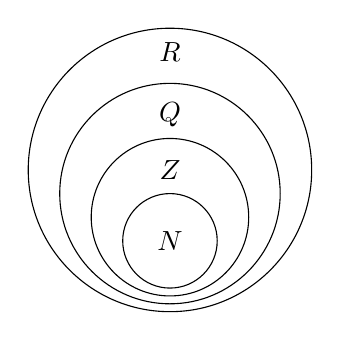
\begin{tikzpicture}
\draw (0.0,0.0) circle (0.6);
\draw (0.0,0.3) circle (1);
\draw (0.0,0.6) circle (1.4);
\draw (0.0,0.9) circle (1.8);
\node at (0,0) {$\mathbb{N}$};
\node at (0,0.9) {$\mathbb{Z}$};
\node at (0,1.6) {$\mathbb{Q}$};
\node at (0,2.4) {$\mathbb{R}$};
\end{tikzpicture}
\caption{Inklusionsforhold mellem $\mathbb{N},\mathbb{Z},\mathbb{Q}$ og $\mathbb{R}$.}
\label{fig:venn1}
\end{figure}
Fig. \ref{fig:Maengdeop} beskriver mængdeoperationer med Venn-diagrammer. 
\begin{figure}[H]


 \centering
 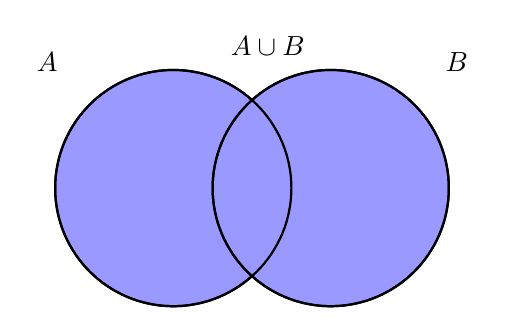
\begin{tikzpicture}[thick,
    set/.style = { circle, minimum size = 3cm}]

\draw[fill=blue!40] (0,0) circle (1.5cm);
\draw[fill = blue!40] (2,0) circle (1.5cm);
\draw[] (0,0) circle (1.5cm);
\draw (2,0) circle (1.5cm);

\node at (1.2,1.8) {$A\cup B$};
\node at (-1.6,1.6) {$A$};
\node at (2+1.6,1.6) {$B$};
\end{tikzpicture}
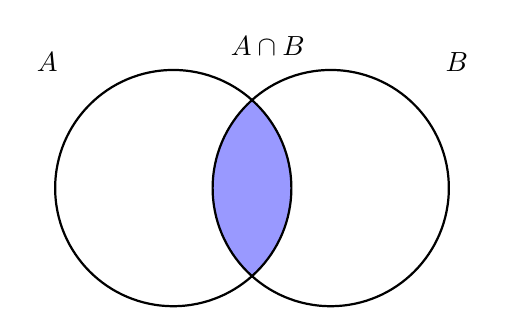
\begin{tikzpicture}[thick,
    set/.style = { circle, minimum size = 3cm}]


\node at (1.2,1.8) {$A\cap B$};
\node at (-1.6,1.6) {$A$};
\node at (2+1.6,1.6) {$B$};

\begin{scope}
    \clip (0,0) circle(1.5cm);
    \clip (2,0) circle(1.5cm);
    \fill[blue!40](0,0) circle(1.5cm);
\end{scope}
\draw[] (0,0) circle (1.5cm);
\draw[] (2,0) circle (1.5cm);
\end{tikzpicture}

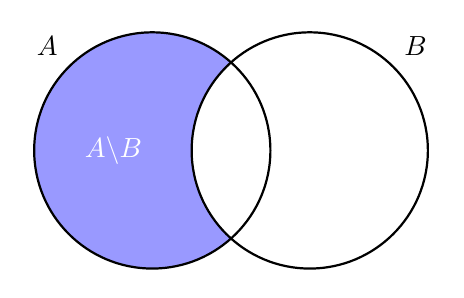
\begin{tikzpicture}[thick,
    set/.style = { circle, minimum size = 3cm}]
 
% Set A
\node[set,fill=blue!40,label={135:$A$}] (A) at (0,0) {};
 
% Set B
\node[set,fill=white,label={45:$B$}] (B) at (0:2) {};
 
% Circles outline
\draw (0,0) circle(1.5cm);
\draw (2,0) circle(1.5cm);
 
% Difference text label
\node[left,white] at (A.center){$A \backslash B$};
 
\end{tikzpicture}
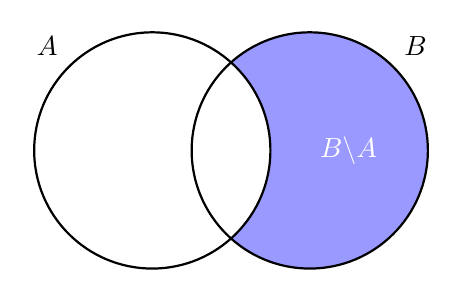
\begin{tikzpicture}[thick,
    set/.style = { circle, minimum size = 3cm}]
 
% Set B
\node[set,fill=blue!40,label={45:$B$}] (B) at (0:2) {};
 
% Set A
\node[set,fill=white,label={135:$A$}] (A) at (0,0) {};
 
% Circles outline
\draw (0,0) circle(1.5cm);
\draw (2,0) circle(1.5cm);
 
% Difference text label
\node[right,white] at (B.center){$B\backslash A$}; 
\end{tikzpicture}
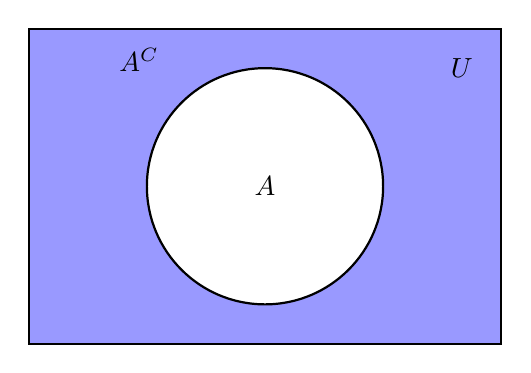
\begin{tikzpicture}[thick,
    set/.style = { circle, minimum size = 3cm}]
\draw[fill = blue!40] (-3,0) rectangle (3,4);
\draw[fill = white] (0,2) circle (1.5cm);

\node at (2.5,3.5) {$U$};
\node at (0,2) {$A$};
\node at (-1.6,1.6+2) {$A^C$};
\end{tikzpicture}
\caption{Mængdeoperationer beskrevet med Venn-diagrammer}
\label{fig:Maengdeop}
\end{figure}

\section*{Opgave 1}
Bestem følgende mængder:
\begin{align*}
&1) \ \{7,9\} \cup \{9,4\}  &&2) \ \{1,3\} \backslash \{1,3\}    \\
&3) \ \{\emptyset, \{\emptyset\}\} \cap \{\{\emptyset\}\}  &&4) \ \{1,2,3\} \cap \{3,4,5\}  \\
&5) \ \{a,b,c\} \cup \{c,d,e\}  &&6) \ \{a,b,c\} \cap \{c,d,e\}   \\
\end{align*}
\section*{Opgave 2}
Opskriv eksemplerne fra noterne som Venn-diagrammer
\section*{Opgave 3}
\begin{enumerate}[label=\roman*)]
\item Er mængden af primtal en delmængde af de ulige tal? Hvorfor? Hvorfor ikke?
\item Er de lige tal en delmængde af de hele tal? Hvad med de ulige tal? Hvorfor? Hvorfor ikke?
\end{enumerate}
\section*{Opgave 4}
Potensmængden $\mathbb{P}(A)$ består af mængden af alle delmængder af $A$. Husk, at den tomme mængde er indeholdt i alle mængder. Opskriv følgende potensmængder
\begin{align*}
&1) \ \mathbb{P}(\{1,2\})    &&2) \  \mathbb{P}(\{1,2,3\})  \\
&3) \ \mathbb{P}(\{2,4,6,8\})   &&4) \ \mathbb{P}(\{a,b,c\}) \\    
\end{align*}
Hvor mange elementer er der i en potensmængde af en mængde med $n$ elementer?
\section*{Opgave 5}
De Morgans love for mængder lyder: For mængder $A$ og $B$ og universalmængde $U$ gælder der, at
\begin{align*}
(A\cup B)^C = A^C \cap B^C
\end{align*} og
\begin{align*}
(A \cap B)^C = A^C \cup B^C.
\end{align*}
\begin{enumerate}[label=\roman*)]
\item Brug Venn-diagrammer til at overbevise dig om, at De Morgans love er rigtige
\item Bevis De Morgans første lov ved at vise, at $(A\cup B)^C \subseteq A^C \cap B^C$ og $ A^C \cap B^C \subseteq (A\cup B)^C$. (Hint: Antag, at $a \in (A\cup B)^C$ og vis, at $a \in A^C \cap B^C $ og vice versa.)
\end{enumerate}